\section{Post-training}

\begin{takeaway}[title={Takeaway}]
\begin{itemize}[leftmargin=2em]
\item[(1)] Applying \textbf{complementary masking} and a \textbf{mask ratio bandwidth} during SFT improves sample efficiency and stabilizes convergence.
\item[(2)] An auxiliary \textbf{confidence loss} is incorporated to sharpen predictions, which is crucial for efficient parallel decoding.
\item[(3)] \textbf{DPO} is adapted by defining sequence log-probabilities over masked tokens, enabling effective preference alignment for the diffusion model.
\end{itemize}
\end{takeaway}

\subsection{Supervised Fine-Tuning with Block Diffusion}

Following the pre-training phase, the model is aligned to follow user instructions through supervised fine-tuning (SFT). This is achieved by adapting the diffusion training objective to be conditional on an input prompt, $\bm{c}$. The model is thus trained to generate the desired response $\bm{x}_0$ by minimizing the following loss function:
\begin{equation}\label{eq:sft_loss}
    \mathcal{L}_{\text{SFT}}(\theta) = - \mathbb{E}_{t,(\bm{c},\bm{x}_0),\bm{x}_t} \left[\frac{\alpha_{t}'}{1-\alpha_{t}}\sum^{K}_{k=1}\sum_{i=1}^{L_{B}}\mathbb{1}[x_{t,k}^i=\text{[MASK]}]\log p_{\theta}(x^i_{0,k} |\bm{c}, \bm{x}_{0,<k}, \bm{x}_{t,k})\right].
\end{equation}
Here, the model $p_{\theta}$ learns to predict the original tokens $x^i_{0,k}$ of a clean response from a noisy version $\bm{x}_t$. The loss is computed only on masked tokens within the current noisy block $\bm{x}_{t,k}$. To do this, the prediction is conditioned on the prompt $\bm{c}$, auto-regressive context from prior clean blocks $\bm{x}_{0,<k}$, and the current noisy block $\bm{x}_{t,k}$ that it must denoise.

\paragraph{Padding strategies \& Mask ratio bandwidth}
To ensure compatibility with our block-wise attention mask, we quantize each sequence's length. Specifically, the original length is rounded up to the nearest multiple of the block size, $b$. This process defines an "effective length" for each sequence, guaranteeing its boundaries align perfectly with the block boundaries required by the attention mechanism.

To optimize the training dynamics, we further implement a ``mask ratio bandwidth'' strategy. Standard discrete diffusion processes typically sample mask probabilities across the full unit interval, $\alpha_{t} \sim U[0, 1]$. However, as identified by~\cite{Blockdiffusion2025}, extreme masking rates induce high gradient variance while offering minimal learning signal: near-zero masking renders reconstruction trivial, while near-total masking reduces the objective to simply learning data marginals. To mitigate this, we clip the noise schedule, constraining the sampling of mask rates to a bounded interval $[\alpha_{\min}, \alpha_{\max}]$ rather than the full range. This bandwidth restriction focuses the training objective on the noise regimes that provide the most informative gradients, thereby stabilizing convergence and improving the model's generative perplexity.

\paragraph{Complementary Masking}
Complementary Masking~\citep{li_lavida_2025} is a training optimization that enhances the data efficiency of the MDLM objective, $\mathcal{L}_{\text{MDLM}}(\theta)$. The strategy's core principle is to generate two antithetical training instances from a single source sequence $\bm{x}_0$. A primary noised sequence, $\bm{x}_t$, is formed using a random mask, while a complementary sequence, $\bm{x}'_t$, is simultaneously produced using that mask's logical inverse\footnote{We also try complementary masking in CPT and find it only works fine on corpus less than 100B tokens, while it does not show advantages with more training data, so that we only adopt it in post-training.}.

By incorporating both $\bm{x}_t$ and $\bm{x}'_t$ into the same training batch, this method provides a deterministic guarantee: every token position across the sequence length $L$ is presented to the model in its uncorrupted state exactly once within the pair. This not only doubles the effective data utilization from each sample, thereby accelerating convergence, but also entirely eliminates token-level sampling bias. Consequently, the model benefits from a more comprehensive and uniform learning signal at every optimization step, leading to enhanced robustness.

\paragraph{Data Recipe Curation}
A balanced, high-quality SFT dataset underpins the model's capabilities, achieved through a strategic composition of tasks spanning three principal pillars: Reasoning, General, and Industrial. The Reasoning pillar hones analytical and logical faculties through mathematics and code generation. The General pillar cultivates linguistic richness and social intelligence via creative and dialogic tasks. The Industrial pillar embeds domain-specific expertise by simulating end-to-end workflows under real-world constraints. This integrated methodology ensures a holistic skill profile, preventing capability skew and enabling fluid shifts between abstract reasoning and applied problem-solving.

\subsection{Confidence-Aware Parallel Training}

To enhance the model's predictive confidence, which is crucial for 
efficient parallel decoding, we propose Confidence-Aware Parallel (CAP) Training. We incorporate an auxiliary confidence 
loss, $\mathcal{L}_{\text{conf}}$, inspired by dParallel~\citep{chen_dparallel_2025}.
The primary objective, $\mathcal{L}_{\text{SFT}}$, ensures correctness but provides diminishing incentive to sharpen the predictive distribution for tokens that are already correctly predicted. The confidence loss addresses this by selectively minimizing the entropy of the model's output distribution, $p_{\theta}(\bm{x}_0 | \bm{x}_t, \bm{c})$, but only for the subset of tokens that are correctly predicted in a given step. This compels the model to increase its certainty on its correct predictions.
The final training objective is a weighted combination of the two losses:
\begin{equation}\label{eq:dparallel}
\mathcal{L}(\theta) = \mathcal{L}_{\text{SFT}}(\theta) + \lambda \mathcal{L}_{\text{conf}}(\theta),
\end{equation}
where $\lambda$ is a hyperparameter that balances the two objectives. As illustrated in Figure~\ref{fig:tps_tparallel}, CAP training effectively improves the decoding efficiency of LLaDA2.0-flash while maintaining competitive compression performance, demonstrating a favorable trade-off between generation quality and inference speed.

\begin{figure}
    \centering
    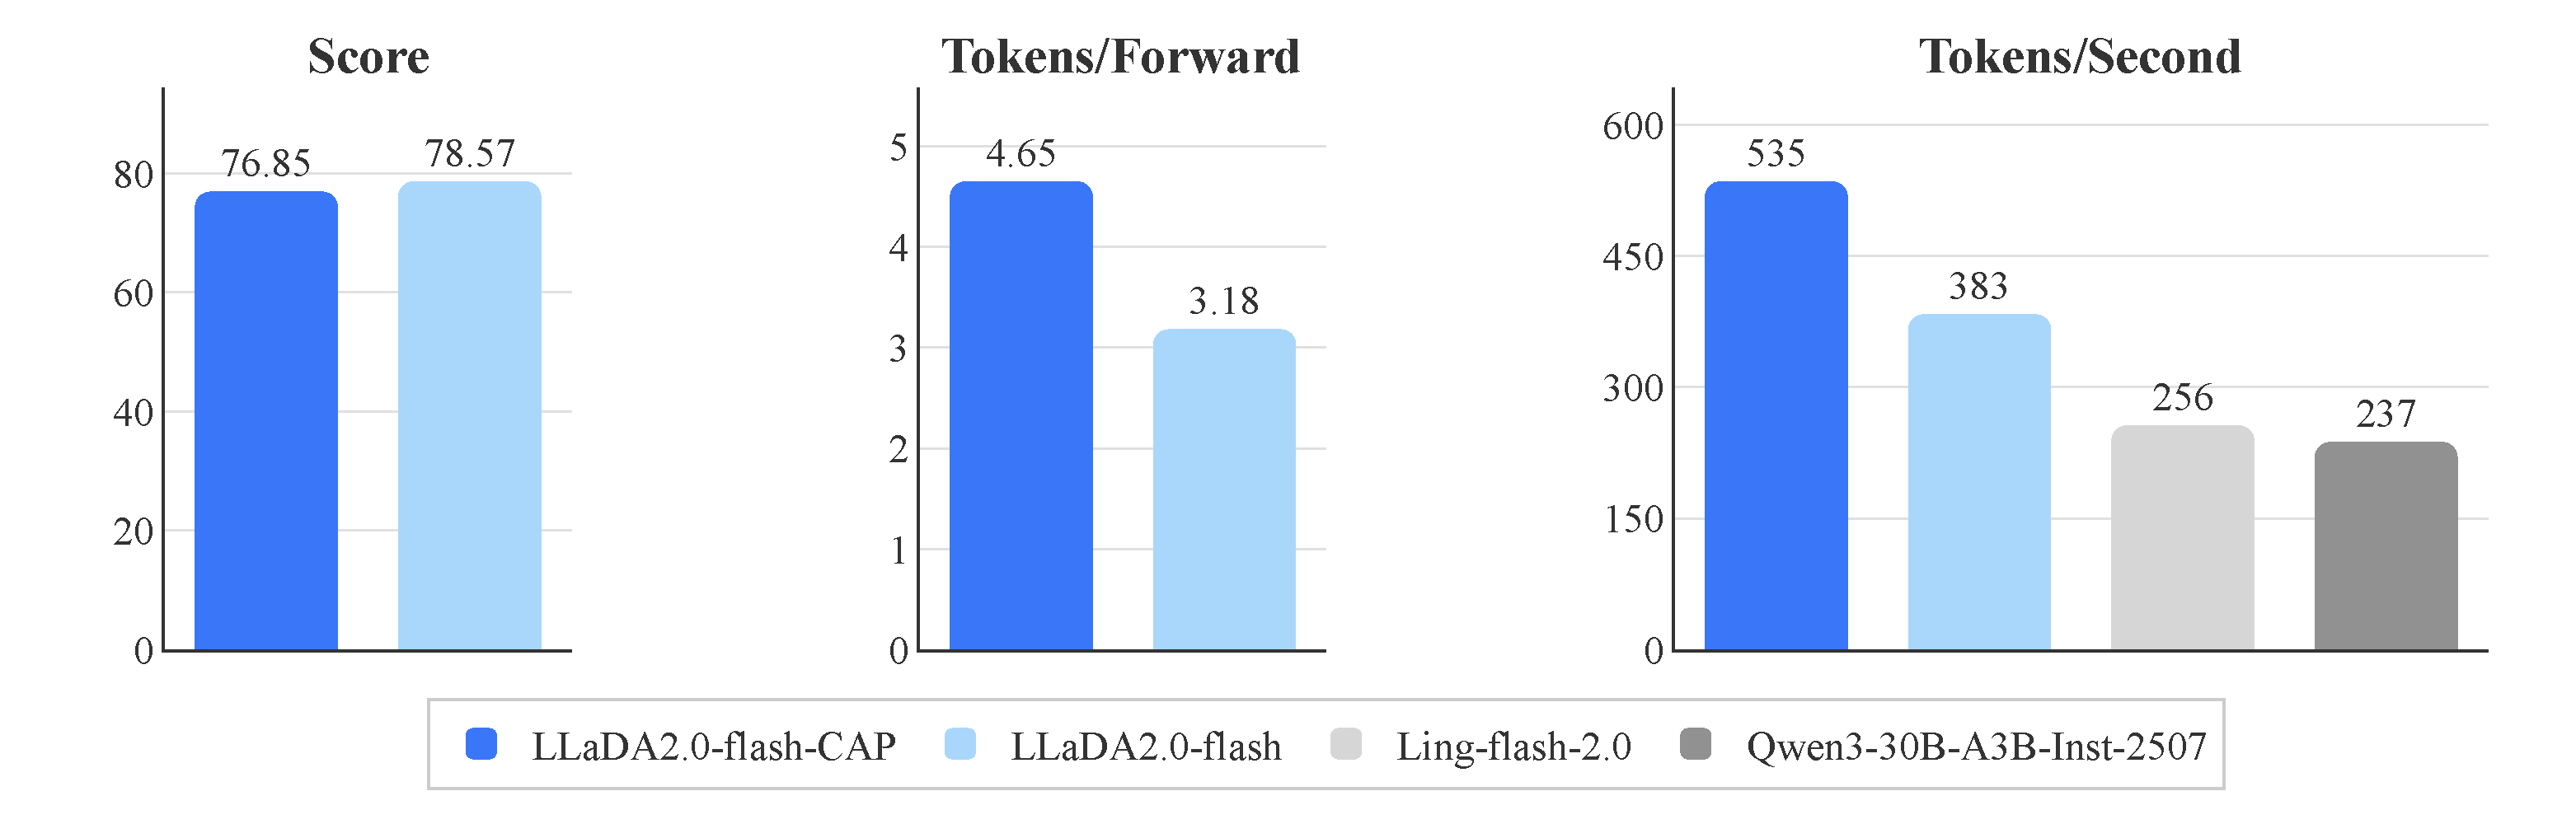
\includegraphics[width=0.95\linewidth]{images/llada2_despine_comparison}
    \caption{Average score and tokens‑per‑forward (TPF) for LLaDA2.0‑flash with and without CAP across 12 benchmarks. Inference speed (tokens per second) of LLaDA2.0‑flash compared with similarly sized AR models on 4 code and math benchmarks.}
    \label{fig:tps_tparallel}
\end{figure}

\subsection{DPO}

Building upon the SFT stage, we further align the policy model $\pi_{\theta}$ with human intent using Direct Preference Optimization. To support this, we constructed a comprehensive dataset comprising 1.5 million preference pairs across diverse domains, including general knowledge, mathematics, and instruction following. To ensure a stable transition in optimization, the learning rate for the DPO stage is initialized consistently with the final learning rate of the preceding SFT phase.

Since the policy model $\pi_{\theta}$ is trained to reconstruct clean tokens $\bm{x}_0$ from noisy blocks $\bm{x}_t$ conditioned on context $\bm{c}$, the standard DPO formulation—which requires exact log-likelihoods—is intractable. Following established practices for diffusion models, we substitute the conditional log-likelihoods with their ELBO. 
We first define the conditional Block Diffusion ELBO, $B_{\text{BDLM}}(\theta, \boldsymbol{x} | \boldsymbol{c})$, for a response $\boldsymbol{x}$. This term mirrors the inner objective of our SFT loss (\eqref{eq:sft_loss}) and is estimated via a single Monte Carlo sample over timesteps and noise:
\begin{equation}\label{eq:bdlm_elbo}
    B_{\text{BDLM}}(\theta, \boldsymbol{x} | \boldsymbol{c}) = \mathbb{E}_{t, \bm{x}_t} \left[ \frac{\alpha_{t}'}{1-\alpha_{t}}\sum_{k=1}^{K} \sum_{i=1}^{L_B} \mathbb{1}[x_{t,k}^i=\text{[MASK]}] \log p_{\theta}(x^i_{k} | \boldsymbol{c}, \boldsymbol{x}_{<k}, \boldsymbol{x}_{t,k}) \right].
\end{equation}
Given a preference pair $(\boldsymbol{x}_w, \boldsymbol{x}_l)$, where $\boldsymbol{x}_w$ is the preferred response and $\boldsymbol{x}_l$ is the dispreferred response, the DPO objective maximizes the margin between the ELBO estimates of the policy $\pi_{\theta}$ and the frozen reference model $\pi_{\theta_{\text{ref}}}$ (initialized from the post-SFT model). The final loss function is defined as:
\begin{equation}\label{eq:dpo_loss}
\mathcal{L}_{\text{DPO}}(\theta) = - \mathbb{E}_{(\boldsymbol{c}, \boldsymbol{x}_w, \boldsymbol{x}_l) \sim \mathcal{D}} \left[ \log \sigma \left( \beta \left[ \Delta B(\boldsymbol{x}_w | \boldsymbol{c}) - \Delta B(\boldsymbol{x}_l | \boldsymbol{c}) \right] \right) \right],
\end{equation}
where $\Delta B(\boldsymbol{x} | \boldsymbol{c}) = B_{\text{BDLM}}(\theta, \boldsymbol{x} | \boldsymbol{c}) - B_{\text{BDLM}}(\theta_{\text{ref}}, \boldsymbol{x} | \boldsymbol{c})$ represents the ELBO advantage of the policy over the reference model, and $\beta$ is a hyperparameter (set to 0.1) that controls the deviation from the reference policy.

\subsection{Inference}
We sample one block at a diffusion step, conditioned on previously sampled blocks $p_{\theta}(\bm{x}^{b}_{s}|\bm{c},\bm{x}^{<b}_{t})$. The generation of each block is itself a multi-step iterative refinement process. At each step, candidate tokens are sampled for all remaining unfilled positions within the block. A hybrid acceptance strategy is then employed: we first accept all tokens whose sampling probability exceeds a predefined confidence `threshold`. If an insufficient number of tokens meet this criterion, a low-confidence fallback is triggered, where we instead accept a fixed number of the most probable tokens regardless of their absolute confidence. This dual mechanism ensures steady generation progress.
